\section{Object Detection with YOLO}
YOLO (\textbf{Y}ou \textbf{O}nly \textbf{L}ook \textbf{O}nce) is a family of single-stage objectors detectors, that got popular for it's detection speed, high accuracy and learning capabilities. YOLO detector pose the object detection problem as a regression problem between bounding boxes and the associated class probabilities \cite{yolov1_paper}.

It is important to note that there are multiple versions such as
YOLOv3 \cite{yolov3_paper}, YOLOv4 \cite{yolov4_paper} and YOLOv7 \cite{yolov7_paper}, but each version may also have multiple implementations e.g. for YOLOv3 there is the Darknet implementation \cite{darknet_git} and also the implementation by Ultralytics \cite{yolov3_ultralytics_git}. One established implementation, that proved good results with a huge community and many features, is the Ultralytics YOLOv5 implementation \cite{yolov5_git}.


\subsection{YOLO architecture}
TODO: Compare YOLO versions in a nutshell \\
TODO: YOLOv5 architecture overview with sizes

\subsection{Labels}
When it comes to labeling of the images, YOLO detectors generally use a distinctive format that consists of 5 numbers for each bounding box: \textit{x, y, w, h, c}. The first two numbers \textit{(x, y)} are the coordinates of the center of the bounding box, then the next two numbers \textit{(w, h)} are the width and height of the bounding box, and finally \textit{c} is the class of the label. The coordinates \textit{(x, y)} and sizes \textit{(w, h)} are normalized w.r.t. the width and height of the image, hence the bounding boxes will always be valid as long the image keeps the same ratio. Each version might have a slight variation of this notation format, but conceptually they are all the same.

\begin{figure}[h]
  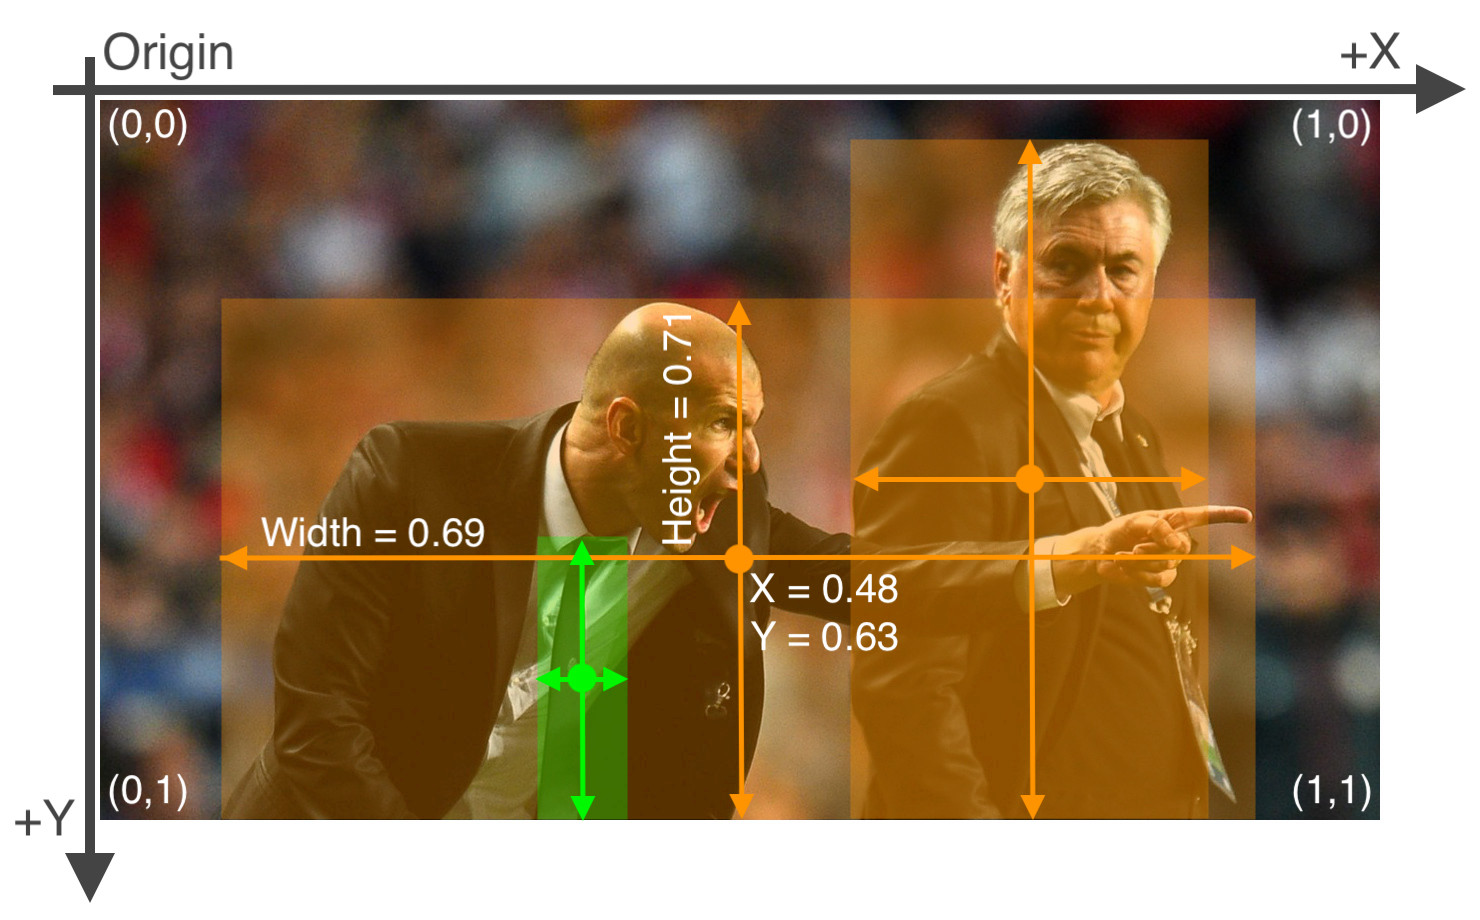
\includegraphics[width=\textwidth]{images/yolo_labels_zidane}
  \centering
  \caption{Example of YOLO bounding box \cite{yolov5_train_custom}}
\end{figure}



\subsection{Metrics \& Benchmarks}
In this section some key concepts regarding the evalution of detections will be defined in order to avoid any sort of confusion and then the evaluation metrics will be presented. \\
The first key concept is the Intersection over Union (IoU), which expresses, how good the overlap between a detection and ground truth bounding box is. The IoU divides the overlap area by the union area, as visualized in figure \ref{fig:iou}.

\begin{figure}[h!]

  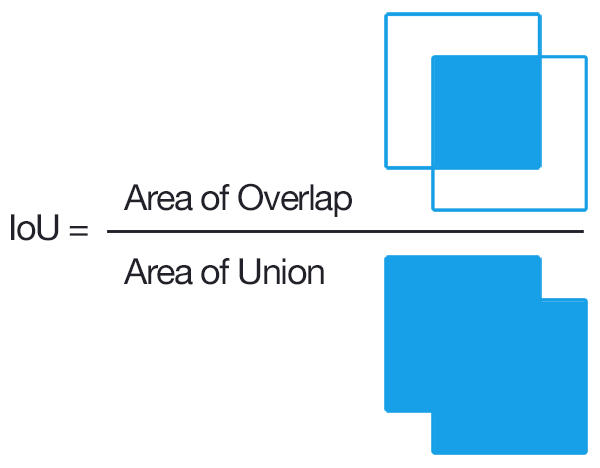
\includegraphics[width=0.75\textwidth]{images/iou}
  \centering
  \caption{IoU formula \cite{map_tutorial}}
  \label{fig:iou}
\end{figure}

The second key concept is the classification of detections in true positive, false positive, false negative. This can be done by taking each detection and seeing, if it has a high IoU with a ground truth bounding box. For a high IoU (i.e. $IoU \geq 0.5$) , then the detection is considered a true positive, else it's a false postive. If a ground truth bounding box is not overlapped by any detections, then the respective missing detection is classified as false negative.\\
Now the metrics precision and recall can be defined:
\begin{equation}
p(c,i) = \frac{TP}{TP + FP}
\end{equation}
\begin{equation}
r(c,i) = \frac{TP}{TP + FN}
\end{equation}
where:
\begin{itemize}
\item[-]{TP = true positives count}
\item[-]{FP = false positives count}
\item[-]{FN = false negatives count}
\item[-]{c = threshold for the confidence of the detections}
\item[-]{i = threshold for the IoU values}
\end{itemize}

The $c$ parameter can be adjusted to improve the recall or precision, which makes sometimes the comparison between two models unclear. Setting the same $conf$ in order to compare two models seems a good approach, but this naive approach might not work, if the models have very different distributions of the confidence values e.g. one model is overconfident and the other one is underconfident. \\
In YOLOv5, this problem was solved by calculating for each model the precision and recall based on the confidence that maximizes the F1-score  \cite{yolov5_conf}:

\begin{equation}
F1(c,i) = 2 * \frac{ p(c,i) * r(c,i)}{p(c,i) + r(c,i)}
\end{equation}

This way a manipulation of the threshold of the confidence values can be avoided and therefor a fairer comparison between models is guaranteed. One caveat of this approach is the assumption that precision and recall have the same importance e.g. an autonomous car needs a higher recall at the detection of red lights. Another caveat of this approach is that it reduces the performance of the model to a single threshold value, but the mean average precison ($mAP$) can be used to express a more general performance. \\
As the name suggests, the $mAP$ is based on the average precision ($AP$), which is calculated indivudually for each class. The AP for a class $C$ and a IoU threshold $i$ can be calculated as follows:

\begin{equation}
AP_C(i) = \sum_{c}{(r(c_{n},i) - r({c_{n-1},i}))p(c_n, i)}
\end{equation}
where $c_n$ are ordered values of confidence thresholds. Finally the mAP is expressed as:
\begin{equation}
mAP(i) = \sum_{C \in classes}{AP_C(i)}
\end{equation}
The IoU threshold can be obviously be lowered to increase the mAP, but usually models are compared for at a threshold of 0.5 and the notation $mAP@0.5$ is preffered. \\
A final metric is the average mAP, usually denoted as $mAP@[0.5:0.95]$. This is just the average $mAP$ for $IoU$ thresholds ranged in 0.5 to 0.95 with a 0.05 step size. \\
For real time object detection application the inference speed is also important
